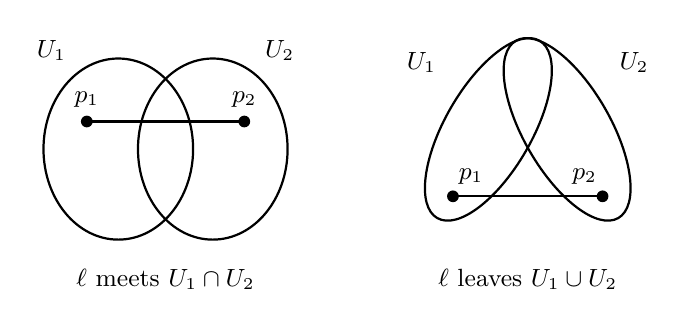
\begin{tikzpicture}[font=\small, dot/.style={circle, fill=black, inner sep=1.5pt}]
% ---------- case 1: the segment passes through U1 \cap U2 ----------
\begin{scope}
  \draw[thick] (0,0) ellipse (0.95 and 1.15);
  \draw[thick] (1.2,0) ellipse (0.95 and 1.15);
  \node at (-0.85,1.25) {$U_1$};
  \node at (2.05,1.25) {$U_2$};
  \draw[thick] (-0.4,0.35) node[dot] (p1) {} -- (1.6,0.35) node[dot] (p2) {};
  \node[above] at (-0.4,0.4) {$p_1$};
  \node[above] at (1.6,0.4) {$p_2$};
  \node[align=center] at (0.6,-1.65) {$\ell$ meets $U_1\cap U_2$};
\end{scope}
% ---------- case 2: the segment avoids U1 \cap U2 ----------
\begin{scope}[xshift=5.2cm, yshift=-0.35cm]
  \draw[thick, rotate around={60:(-0.5,0.6)}] (-0.5,0.6) ellipse (1.3 and 0.55);
  \draw[thick, rotate around={120:(0.5,0.6)}] (0.5,0.6) ellipse (1.3 and 0.55);
  \node at (-1.35,1.45) {$U_1$};
  \node at (1.35,1.45) {$U_2$};
  \draw[thick] (-0.95,-0.25) node[dot] {} -- (0.95,-0.25) node[dot] {};
  \node at (-0.72,0.0) {$p_1$};
  \node at (0.72,0.0) {$p_2$};
  \node[align=center] at (0,-1.3) {$\ell$ leaves $U_1\cup U_2$};
\end{scope}
\end{tikzpicture}
